
\documentclass[aspectratio=169,11pt]{beamer}

%% ─── Columbia palette ────────────────────────────────────────────────────────
\definecolor{cunavy}{HTML}{003865}
\definecolor{cublue}{HTML}{B9D9EB}
\definecolor{cuamber}{HTML}{E67E22}
\definecolor{cugreen}{HTML}{27AE60}
\definecolor{cuslate}{HTML}{2C3E50}
\definecolor{cured}{HTML}{C0392B}
\definecolor{cugrey}{HTML}{7F8C8D}

%% ─── theme ───────────────────────────────────────────────────────────────────
\usetheme{default}
\usecolortheme{default}
\setbeamercolor{frametitle}{fg=white,bg=cunavy}
\setbeamercolor{title}{fg=white}
\setbeamercolor{subtitle}{fg=cublue}
\setbeamercolor{author}{fg=white}
\setbeamercolor{date}{fg=cublue}
\setbeamercolor{structure}{fg=cunavy}
\setbeamercolor{titlelike}{fg=cunavy}
\setbeamercolor{block title}{fg=white,bg=cunavy}
\setbeamercolor{block body}{fg=cuslate,bg=cublue!25}
\setbeamercolor{alerted text}{fg=cuamber}
\setbeamercolor{example text}{fg=cugreen}
\setbeamerfont{frametitle}{size=\large,series=\bfseries}
\setbeamerfont{title}{size=\LARGE,series=\bfseries}
\setbeamerfont{subtitle}{size=\large}
\setbeamertemplate{footline}[frame number]
\setbeamertemplate{navigation symbols}{}
\setbeamertemplate{itemize item}{\textbullet}
\setbeamertemplate{itemize subitem}{--}

\usepackage{graphicx}
\usepackage{booktabs}
\usepackage{xcolor}
\usepackage{amsmath}

\title{Provenance-Aware Stablecoin\\Stress Propagation Networks}
\subtitle{Evidence from Curve TokenExchange Logs, Public CEX Data,\\
          and On-Chain Settlement Flows}
\author{Columbia University MAFN}
\date{May 2026}

\begin{document}

%% ─── title ───────────────────────────────────────────────────────────────────
{\setbeamercolor{background canvas}{bg=cunavy}
\begin{frame}[plain]
\titlepage
\end{frame}
}

\begin{frame}{The Problem: Incomplete Claims About Stablecoin Stress}
\begin{columns}[T]
\column{0.52\textwidth}
\textbf{What happened (2022--2023):}
\begin{itemize}
  \item Terra/LUNA: algorithmic collapse, May 2022
  \item FTX: exchange credit shock, Nov 2022
  \item USDC/SVB: fiat-reserve bank shock, Mar 2023
  \item USDT/Curve: DeFi pool imbalance, Jun 2023
\end{itemize}
\vspace{6pt}
Each episode called ``contagion'' in real time.
\column{0.44\textwidth}
\begin{block}{The data problem}
Most analyses use price data only and treat all sources as equally reliable.\\[4pt]
\textbf{Historical full-depth CEX order books are not freely available} for these episodes.\\[4pt]
Yet microstructure claims are made routinely.
\end{block}
\end{columns}
\end{frame}


\begin{frame}{Stablecoin Stress Is Also a Flow Event}
\begin{columns}[T]
\column{0.50\textwidth}
\textbf{Observable during stress:}
\begin{itemize}
  \item Traders swap in AMM pools \\
        \textcolor{cugreen}{$\to$ Curve \texttt{TokenExchange} logs: \textbf{Tier A}}
  \item Stablecoins minted or burned \\
        \textcolor{cugreen}{$\to$ ERC-20 \texttt{Transfer} logs: \textbf{Tier A}}
  \item Price deviations at CEXs \\
        \textcolor{cugrey}{$\to$ Public OHLCV/BBO: \textbf{Tier B}}
  \item CEX order-book depth \\
        \textcolor{cured}{$\to$ Historical L2: \textbf{not freely available}}
\end{itemize}
\column{0.46\textwidth}
\begin{block}{Key asymmetry}
Curve \texttt{TokenExchange} events are:
\begin{itemize}
  \item Immutable, block-timestamped
  \item Exact amounts per transaction
  \item Freely reproducible from any Ethereum node
\end{itemize}
\vspace{4pt}
\textbf{Public CEX OHLCV is not execution-grade.}
\end{block}
\end{columns}
\end{frame}


\begin{frame}{This Paper: Two Contributions}
\begin{columns}[T]
\column{0.50\textwidth}
\begin{exampleblock}{Contribution 1: Flow-Based Evidence}
Study stablecoin stress as a \emph{liquidity-flow event}, not only a price event.\\[6pt]
Tier-A Curve TokenExchange logs provide execution-grade AMM-flow evidence not available from CEX feeds.
\end{exampleblock}
\column{0.46\textwidth}
\begin{exampleblock}{Contribution 2: Provenance-Aware Gate}
Every empirical edge is filtered by:\\[4pt]
\begin{enumerate}
  \item \textbf{Provenance gate} (data quality tier)
  \item \textbf{Statistical gate} (significance)
  \item \textbf{Paper gate} (both must pass)
\end{enumerate}
\vspace{4pt}
\texttt{paper\_claim\_allowed = True} only when both gates clear.
\end{exampleblock}
\end{columns}
\vspace{8pt}
\centering
\textbf{\color{cuamber}One robust A/A result across 5 events.  The framework tells you exactly why only one.}
\end{frame}


\begin{frame}{Data Architecture: Three Layers, Two Tiers}
\begin{center}
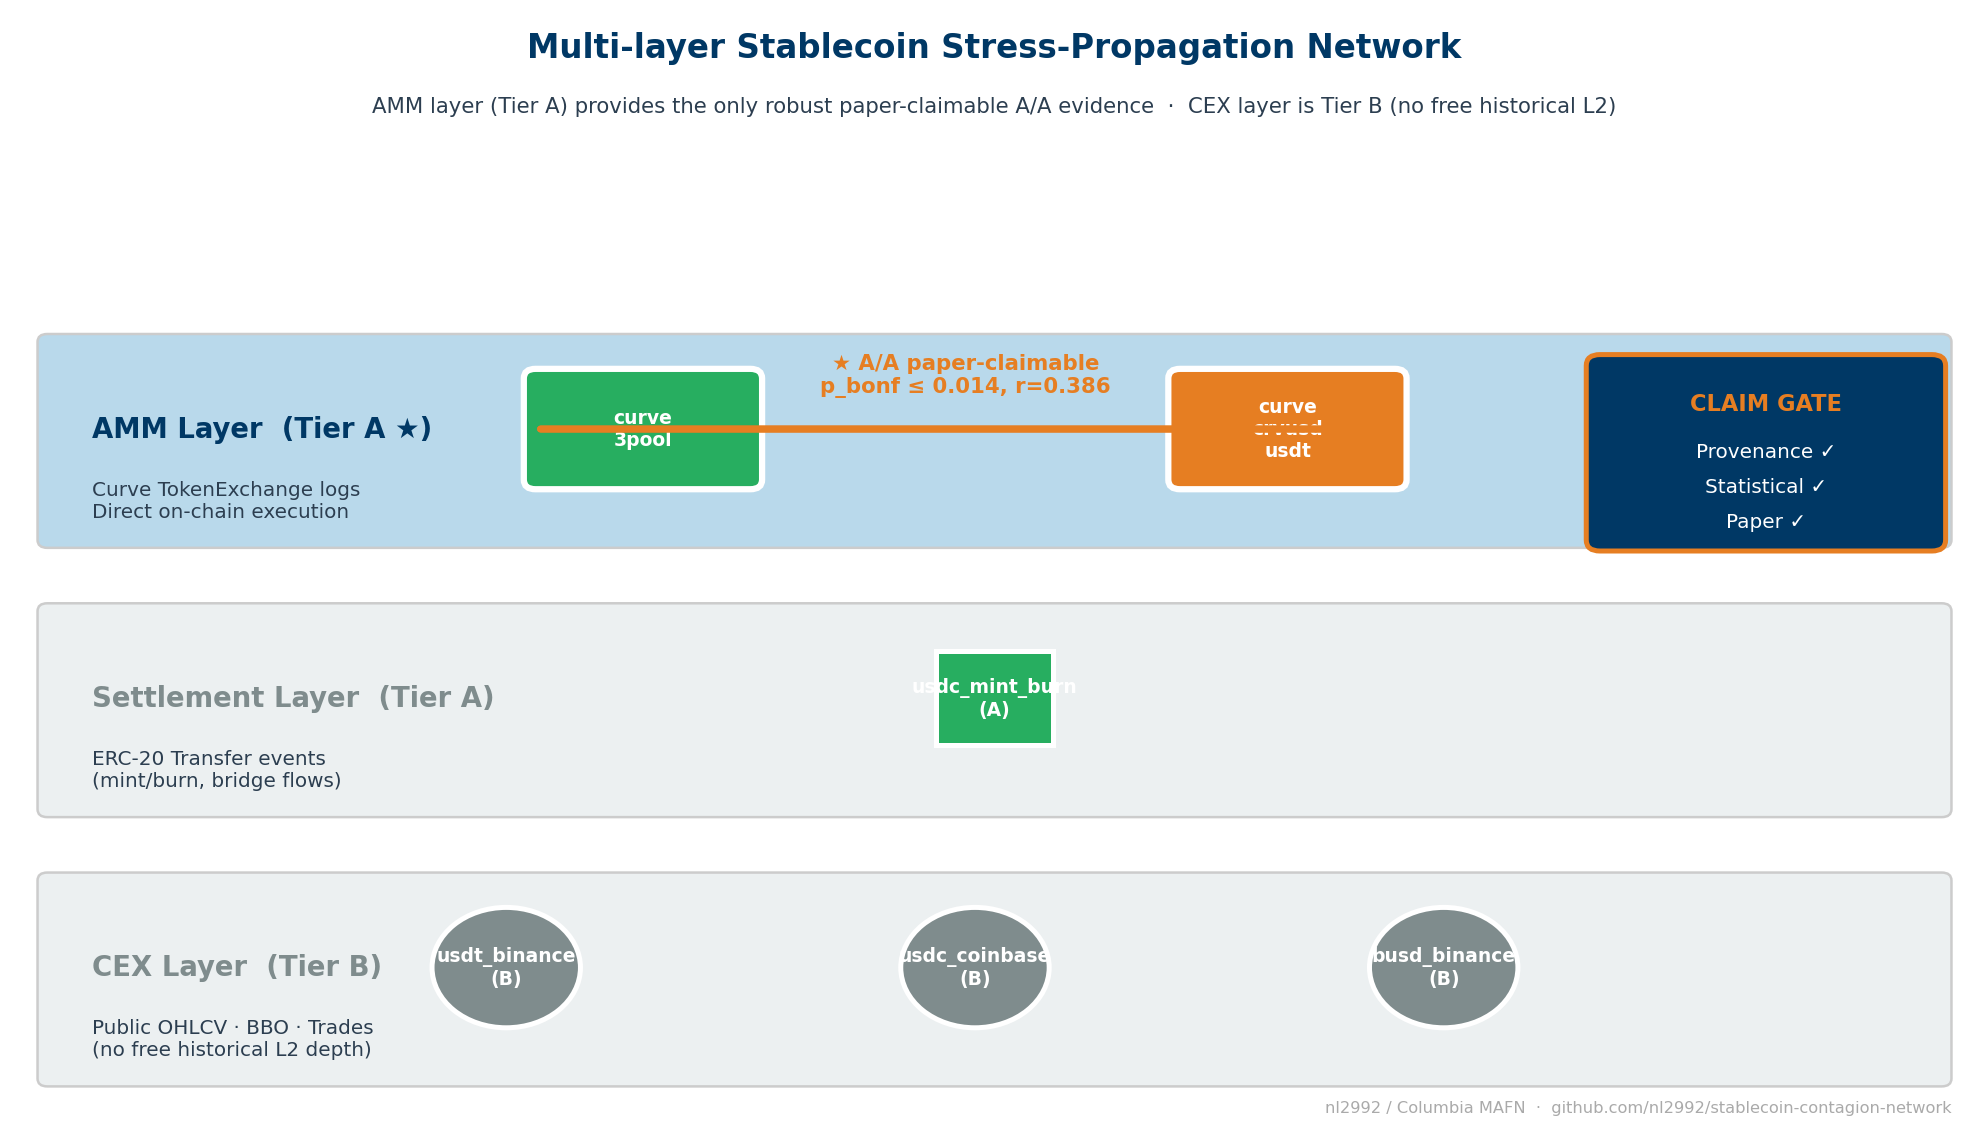
\includegraphics[width=0.78\textwidth]{figures_tex/fig_01.png}
\end{center}
\vspace{-4pt}
{\small
\textcolor{cugreen}{\textbf{Tier A}} --- Curve TokenExchange logs, ERC-20 Transfer events (execution-grade, freely reproducible)\\
\textcolor{cugrey}{\textbf{Tier B}} --- Public CEX OHLCV, BBO, CoinMetrics netflows (context only, no free historical L2)
}
\end{frame}


\begin{frame}{Claim-Gate Pipeline}
\begin{center}
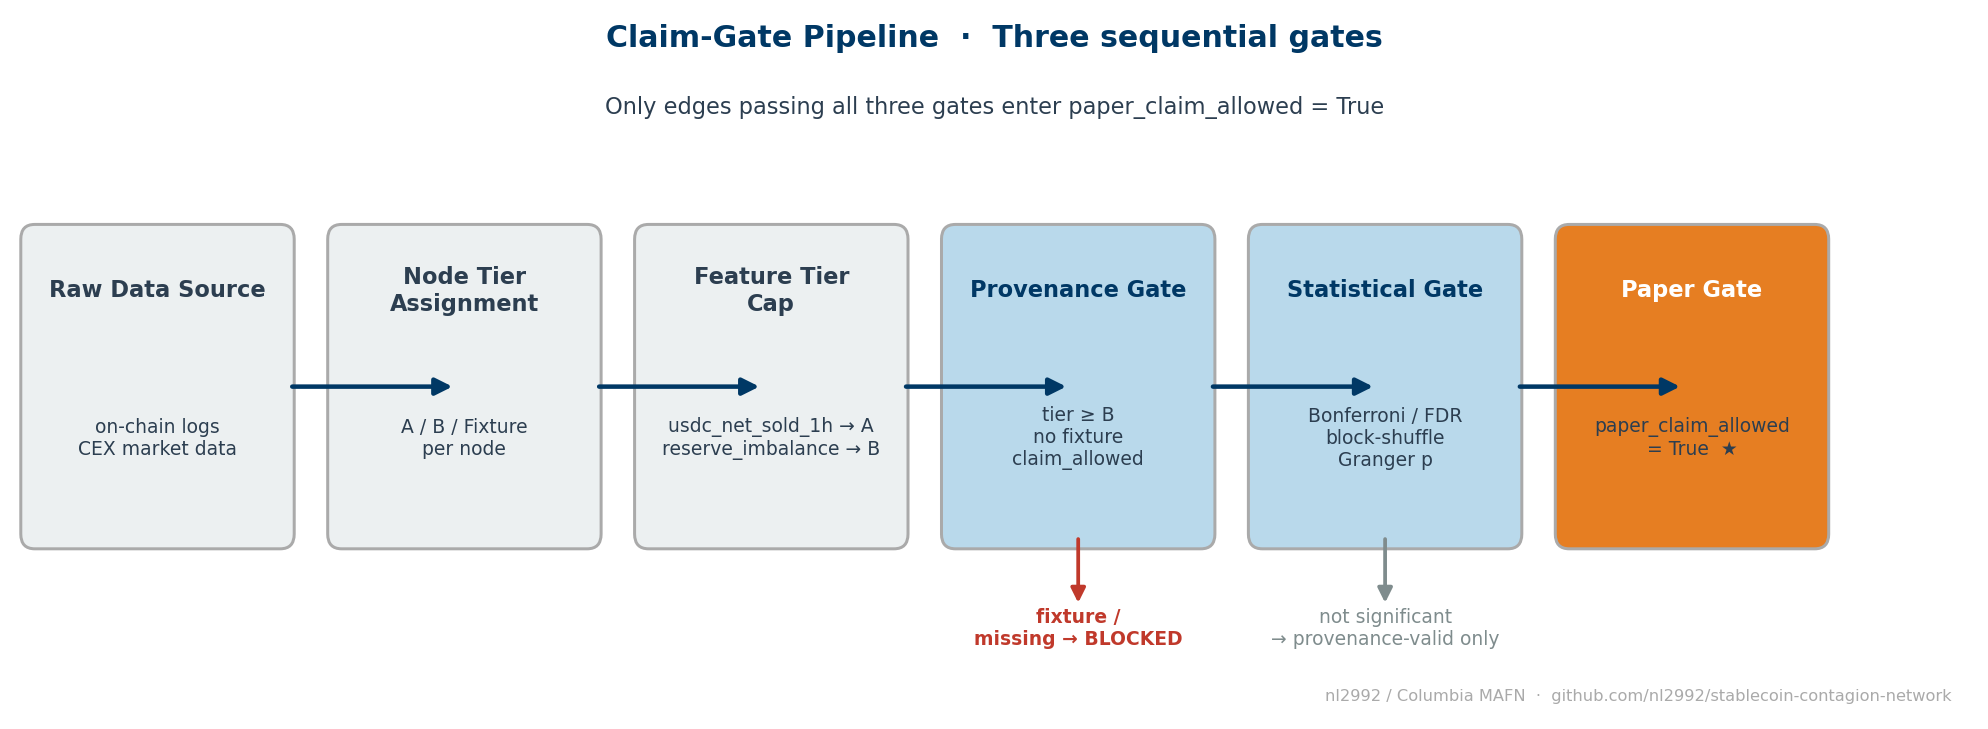
\includegraphics[width=0.82\textwidth]{figures_tex/fig_02.png}
\end{center}
\vspace{-4pt}
{\small
Three sequential gates.  An edge is \textbf{paper-claimable} only if it clears all three.\\
The amber path (A/A DEX-flow) is the only route that reaches \texttt{paper\_claim\_allowed = True} in USDT/Curve 2023.
}
\end{frame}


\begin{frame}{Five Events: What Each Provides}
\centering
\small
\begin{tabular}{lcccl}
\toprule
Event & A/A prov & A/A paper & A/B paper & Status \\
\midrule
\textbf{USDT/Curve 2023} & 6 & \textbf{\textcolor{cugreen}{2}} & 1 & \textcolor{cugreen}{\textbf{Robust headline result}} \\
Terra/LUNA 2022 & 6 & \textcolor{cured}{0} & 4 & Provenance-valid, stat.\ fails \\
USDC/SVB 2023   & 1 & \textcolor{cured}{0} & 4 & Underpowered sparse flow \\
FTX 2022        & 0 & 0 & 5 & A/B contextual only \\
BUSD 2023       & 0 & 0 & 7 & A/B contextual only \\
\bottomrule
\end{tabular}
\vspace{10pt}
\textbf{Provenance-valid $\neq$ paper-claimable.}\\[4pt]
Terra has 6 A/A candidates; zero pass the statistical gate.
\end{frame}


\begin{frame}{Headline Result: USDT/Curve 2023}
\begin{columns}[T]
\column{0.48\textwidth}
\begin{block}{Paper-claimable A/A result}
\centering
\vspace{4pt}
{\LARGE\bfseries\color{cuamber} $\hat{\rho} = 0.386$}\\[6pt]
{\large Bonferroni $p \le 0.014$}\\[6pt]
\texttt{curve\_3pool $\leftrightarrow$ curve\_crvusd\_usdt}\\[4pt]
Feature: \texttt{usdc\_net\_sold\_1h} (Tier A)\\
Grid: hourly $\cdot$ claim: robust
\end{block}
\column{0.48\textwidth}
\textbf{What this means:}
\begin{itemize}
  \item Both pools co-move simultaneously (lag = 0)
  \item Both directions pass Bonferroni
  \item Evidence: Tier-A on-chain logs only
  \item Claim level: A/A DEX-flow
\end{itemize}
\vspace{6pt}
\textbf{\color{cured}What this does NOT mean:}
\begin{itemize}
  \item No structural causal identification
  \item Does not extend to CEX venues
  \item Does not apply to other 4 events
\end{itemize}
\end{columns}
\end{frame}


\begin{frame}{Evidence: Tier-A AMM Flow During USDT/Curve 2023}
\begin{center}
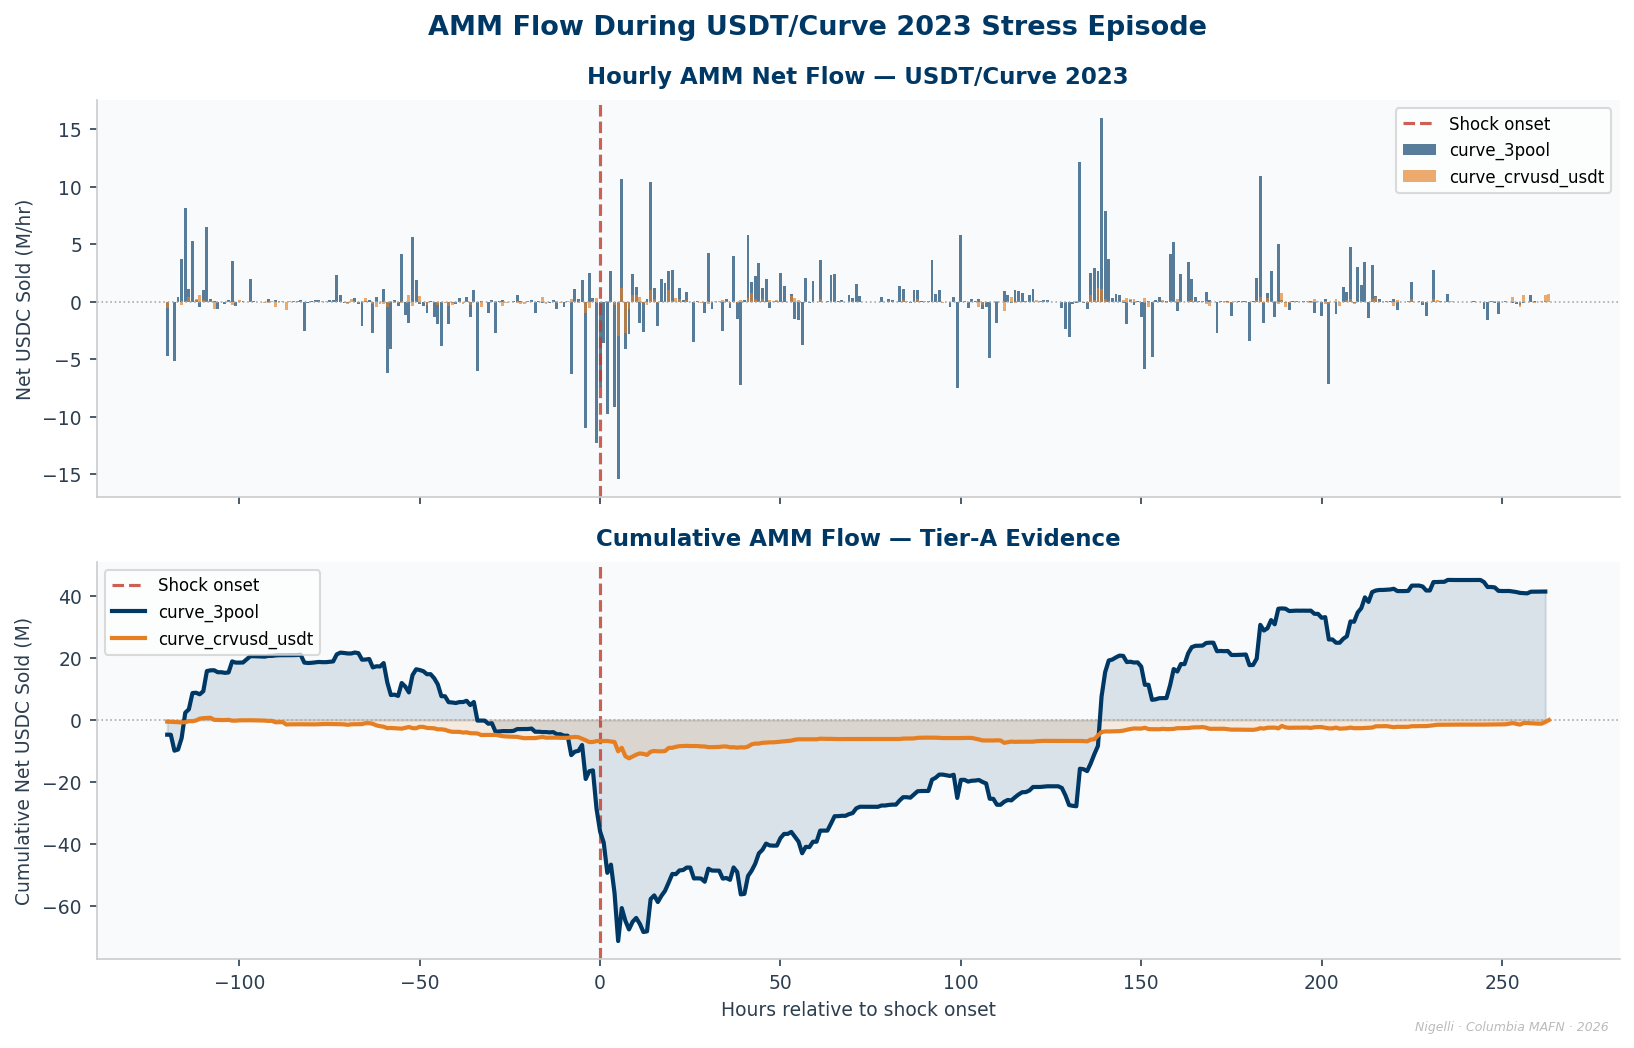
\includegraphics[width=0.88\textwidth]{figures_tex/fig_03.png}
\end{center}
\vspace{-4pt}
{\small
Hourly \texttt{usdc\_net\_sold\_1h} for both Curve pools.
Both pools show elevated net outflows simultaneously around the stress onset (dashed line).
Data: Etherscan \texttt{TokenExchange} logs --- Tier A.
}
\end{frame}


\begin{frame}{Evidence: Lead-Lag Cross-Correlation Profile}
\begin{center}
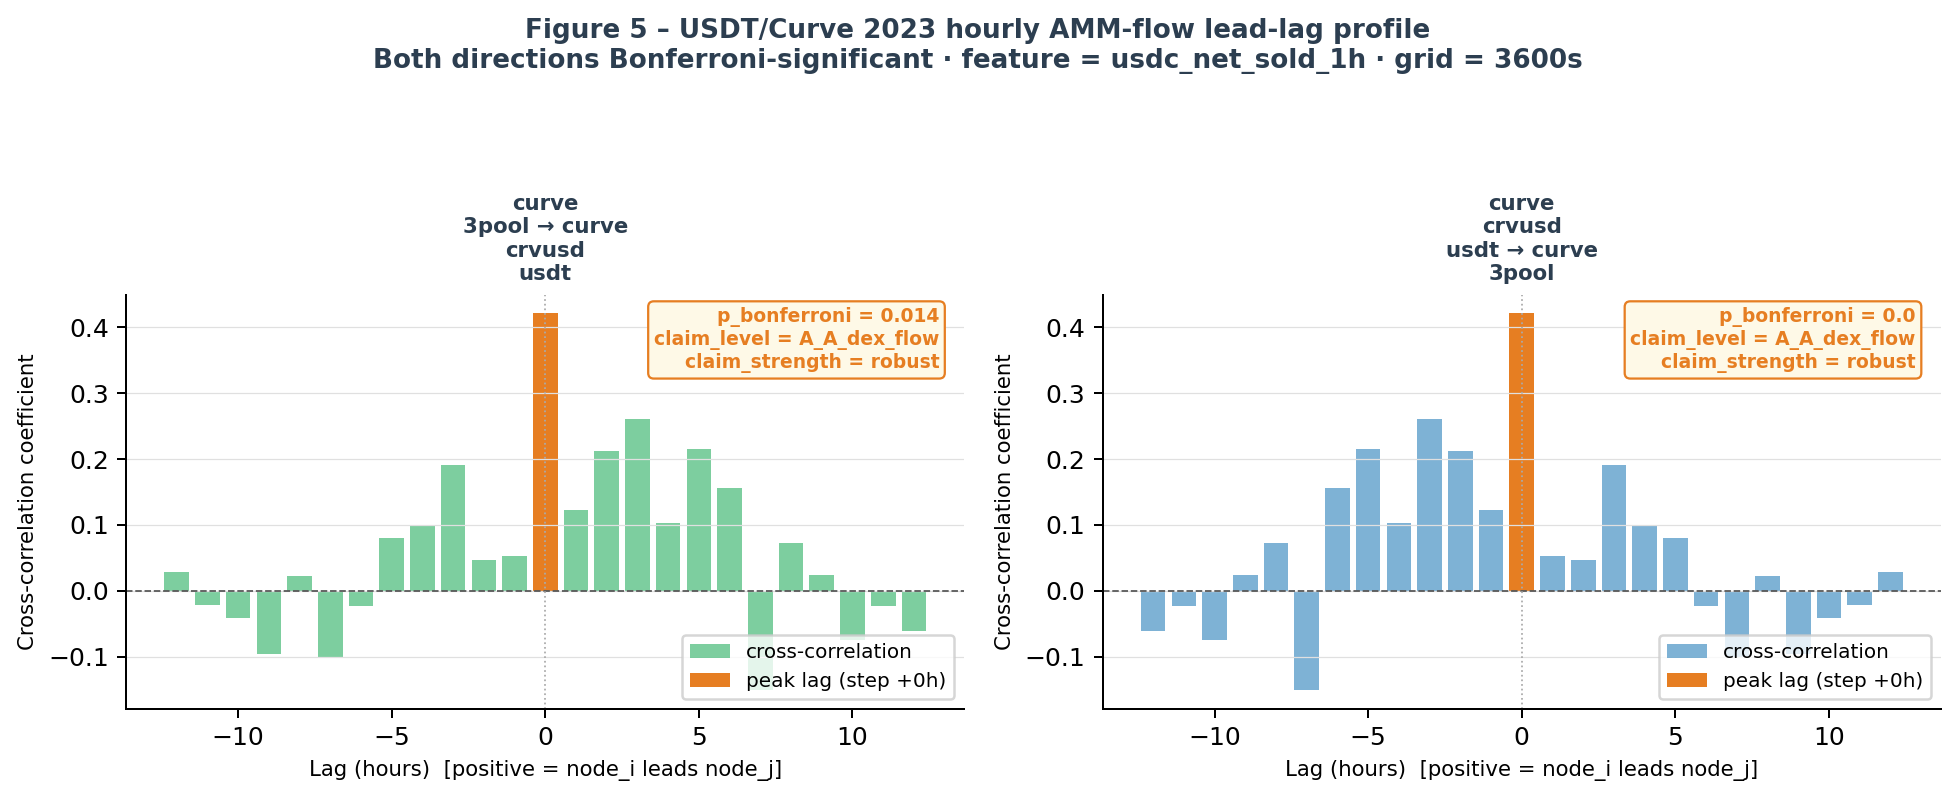
\includegraphics[width=0.70\textwidth]{figures_tex/fig_04.png}
\end{center}
\vspace{-4pt}
{\small
Peak correlation at lag = 0 in both directions.
Horizontal dashed line: Bonferroni significance threshold.
Simultaneous co-movement, not sequential transmission.
}
\end{frame}


\begin{frame}{Cross-Event Evidence Map}
\begin{center}
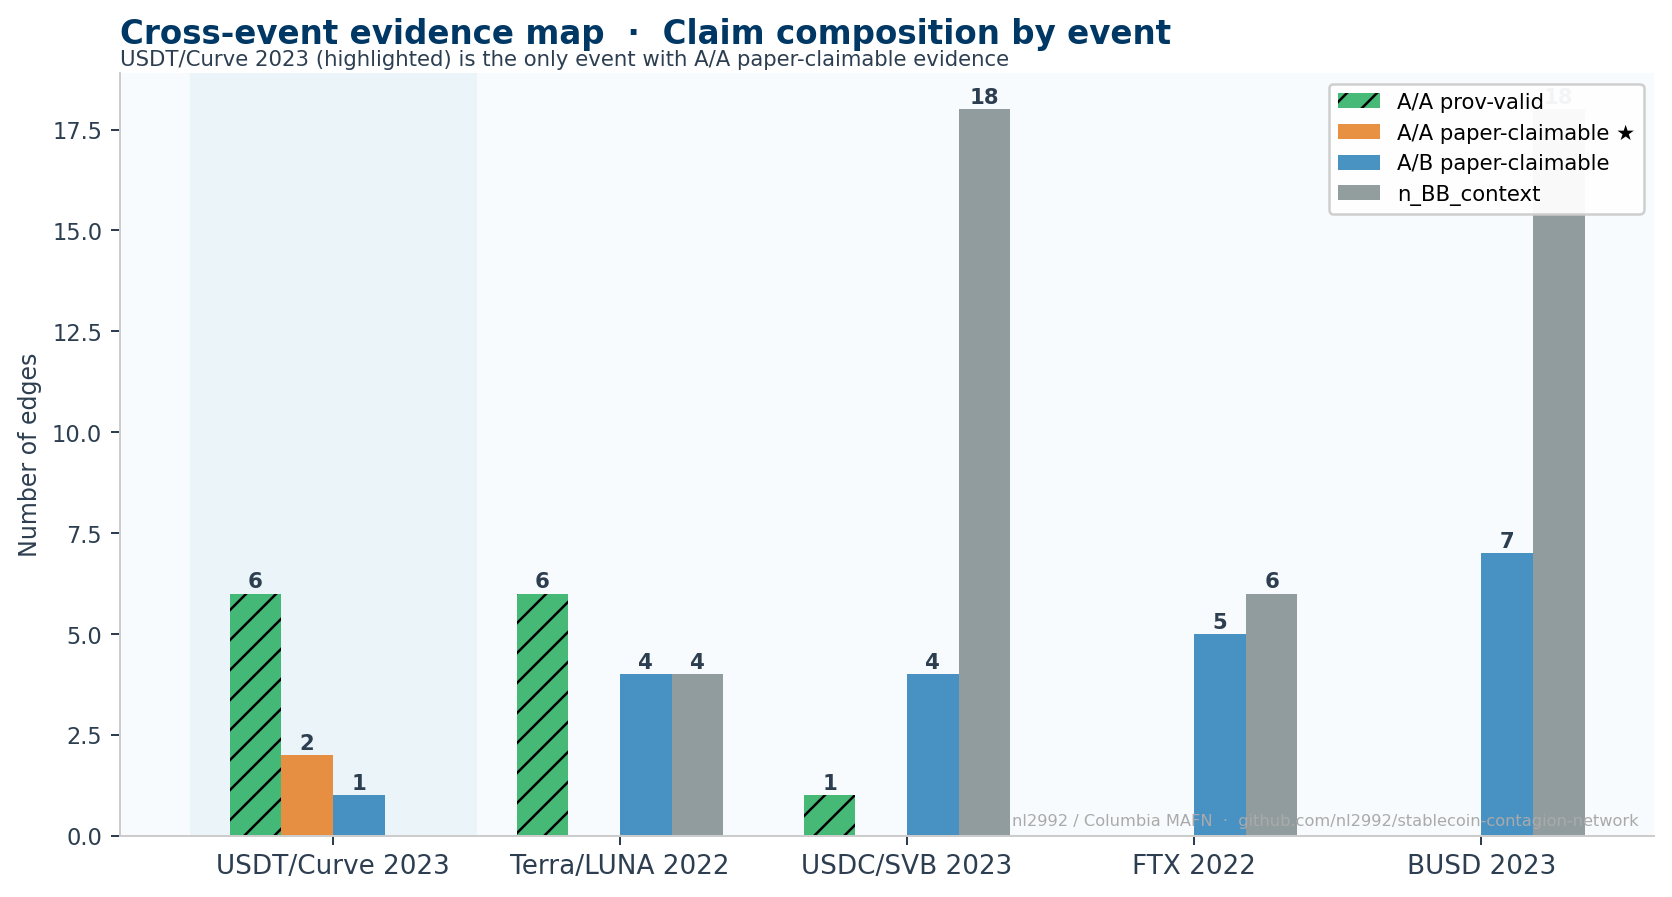
\includegraphics[width=0.82\textwidth]{figures_tex/fig_05.png}
\end{center}
\vspace{-4pt}
{\small
Only USDT/Curve 2023 reaches A/A paper-claimable status (amber).
Terra/LUNA has A/A provenance-valid candidates (grey) that fail the statistical gate.
FTX and BUSD provide A/B contextual evidence only.
}
\end{frame}


\begin{frame}{Terra/LUNA 2022: The Negative Result}
\begin{columns}[T]
\column{0.52\textwidth}
\begin{alertblock}{Not paper-claimable}
Terra/LUNA has \textbf{6 A/A provenance-valid} candidate pairs\\[4pt]
(Curve 3pool $\leftrightarrow$ Curve UST/Wormhole)\\[6pt]
\textbf{Zero pass the statistical gate} at the hourly grid.
\end{alertblock}
\vspace{6pt}
The Terra collapse unfolded over days; hourly resolution may be too coarse to detect the fast dynamics of the algorithmic unwind.
\column{0.44\textwidth}
\begin{block}{Why this matters}
This is not a data problem---it is a genuine statistical finding.\\[6pt]
Reporting negative results is part of the provenance-aware framework.\\[6pt]
\textbf{Provenance-valid $\neq$ paper-claimable.}
\end{block}
\end{columns}
\end{frame}


\begin{frame}{USDC/SVB 2023: Underpowered Settlement Signal}
\begin{columns}[T]
\column{0.52\textwidth}
\textbf{What we observe:}
\begin{itemize}
  \item 4~mint-burn arrival events identified
  \item Mean 3-hour post-arrival response: +\$28,956~USDC (+10.8\%)
  \item Direction consistent with de-peg stress
\end{itemize}
\vspace{6pt}
\begin{alertblock}{Not paper-claimable}
Permutation test $p = 1.00$\\
With only 4~events, the test is severely underpowered.
\end{alertblock}
\column{0.44\textwidth}
\begin{block}{Documented as}
\textbf{Provenance-valid, statistically unsupported} candidate.\\[6pt]
Included in the paper package as a negative result, not a positive claim.\\[6pt]
Motivates future data collection.
\end{block}
\end{columns}
\end{frame}


\begin{frame}{Robustness: Headline Pair Stable Across Grid Configurations}
\begin{columns}[T]
\column{0.52\textwidth}
\textbf{Checked across:}
\begin{itemize}
  \item \texttt{baseline\_60s} --- 1-minute grid
  \item \texttt{block\_300} --- 5-minute block-bootstrap
  \item \texttt{block\_1800} --- 30-minute block-bootstrap
\end{itemize}
\vspace{6pt}
\textbf{Headline pair}: significant across all configurations.\\[4pt]
\textbf{Terra pair}: non-significant across all configurations.
\column{0.44\textwidth}
\begin{block}{Significance rate heatmap}
Green = high significance rate across pairs.\\
Red = low significance rate.\\[4pt]
USDT/Curve 2023 stays green.\\
Terra/LUNA stays red.
\end{block}
\end{columns}
\end{frame}


\begin{frame}{What This Paper Does NOT Claim}
\begin{columns}[T]
\column{0.50\textwidth}
\begin{alertblock}{\textcolor{white}{Blocked claims}}
\begin{itemize}
  \item \textbf{Historical CEX order-book data} from Binance/Kraken/Coinbase
  \item \textbf{CEX execution-grade microstructure} transmission in any event
  \item \textbf{Structural causal identification} from lead-lag or Granger
  \item \textbf{A/A paper-claimable evidence} for Terra, USDC/SVB, FTX, or BUSD
  \item \textbf{Tier-A status} for derived Curve proxies (\texttt{reserve\_imbalance}, \texttt{implied\_pool\_price})
\end{itemize}
\end{alertblock}
\column{0.46\textwidth}
\begin{exampleblock}{Why explicit non-claims matter}
``Does not claim'' is as important as the positive result.\\[6pt]
The claim gate forces discipline: you cannot make a claim your data cannot support.\\[6pt]
All non-claims are verified in the automated validation script.
\end{exampleblock}
\end{columns}
\end{frame}


\begin{frame}{Conclusion}
\begin{columns}[T]
\column{0.52\textwidth}
\textbf{Three takeaways:}
\begin{enumerate}
  \item \textbf{One robust A/A result}\\
    Curve 3pool $\leftrightarrow$ crvUSD/USDT\\
    $\hat{\rho}=0.386$, Bonferroni $p\le0.014$\\
    Tier-A Curve TokenExchange logs, June 2023.
  \vspace{4pt}
  \item \textbf{Provenance matters}\\
    Tier-A AMM flow $\neq$ Tier-B CEX candles.\\
    The gate forces honest accounting.
  \vspace{4pt}
  \item \textbf{Negative results are informative}\\
    Terra has 6 A/A candidates; zero pass.\\
    USDC/SVB signal is real but underpowered.
\end{enumerate}
\column{0.44\textwidth}
\begin{block}{Next steps}
\begin{itemize}
  \item Collect live CEX L2 during future stress events
  \item Extend to Uniswap v3 pools
  \item Higher-frequency mint-burn analysis
  \item Longer event windows for sparse-flow tests
\end{itemize}
\end{block}
\vspace{8pt}
\centering
\textbf{\color{cuamber} Code, data, and validation:\\
\texttt{github.com/nl2992/\\stablecoin-contagion-network}}
\end{columns}
\end{frame}

\end{document}